\documentclass[10pt]{beamer}
\usetheme[]{Feather}
\setbeamercolor{Feather}{fg=black!20,bg=black}
\setbeamercolor{structure}{fg=black}
\usepackage[utf8]{inputenc}
\usepackage[spanish]{babel}
\usepackage[T1]{fontenc}
\usepackage{helvet}
\usepackage{lipsum}
\usepackage{amsmath,amssymb,amsfonts}
\usepackage{amsthm}
\usepackage{physics}
\usepackage{framed, color}
\usepackage{epsfig}
\usepackage{acronym}
\usepackage{multirow, array} 
\usepackage{float}
\usepackage[T1]{fontenc}
\usepackage{natbib}
\usepackage{fancyhdr}
\usepackage{xcolor}
\usepackage{multicol}
\usepackage{mdframed}
\usepackage{endnotes}
\usepackage{listings}
\usepackage{tensor}
\usepackage{csquotes}
\renewcommand{\thefootnote}{\arabic{footnote}}
\newcommand{\chref}[2]{
  \href{#1}{{\usebeamercolor[bg]{Feather}#2}}
}
\title[]
{
      \textbf{Estabilidad y transiciones de fase en el sistema de Lotka-Volterra generalizado.}
}

\subtitle[Tema o materia]
{Examen profesional}

\author[Autor]
{      Rodrigo Vega Vilchis
}
\subtitle{Asesor: Sergio A. Alcalá Corona.}

\institute[]
{
      \large{Facultad de Ciencias}\\
      Universidad Nacional Autónoma de México
  
  %there must be an empty line above this line - otherwise some unwanted space is added between the university and the country (I do not know why;( )
}
\date{}
\begin{document}


\begin{frame}
  \frametitle{Sistema de Lotka-Volterra generalizado}
  Se define el sistema:
  \begin{equation}\label{eqn:LK}
  	\frac{dx_i}{dt}=r_ix_i\left(1-\frac{\sum_{j=1}^N\alpha_{ij}x_j}{K_i}\right)
  \end{equation}
  \begin{itemize}
  	\item donde $r_i$ es la tasa de crecimiento,
  	\item $K_i$ es la capacidad de carga del sistema,
  	\item $x_i$ es la población de una especie y su derivada marca la dinámica de su crecimiento,
  	\item $\alpha_{ij}x_j$ con las especies que interaccionan con $x_i$ con cierto valor $\alpha_{ij}$.
  \end{itemize}  
\end{frame}
\begin{frame}
  \frametitle{Sistema de Lotka-Volterra generalizado}
	  Sea $\textbf{F}:\mathbb{R}^n\to\mathbb{R}^n$, se define su aspecto matricial de la siguiente forma
	  $$\textbf{F}(\vec{x})=\begin{pmatrix}
	  	f_1(\vec{x})\\
	  	\vdots\\
	  	f_n(\vec{x})
	  \end{pmatrix},\qquad\text{donde }\vec{x}=(x_1(t),...,x_n(t))$$   
	  y cada una de las $f_i(\vec{x})$ corresponde con las funciones del sistema (\ref{eqn:LK}). El sistema puede ser re-escrito de la siguiente forma
	  $$\dot{\vec{x}}=\textbf{F}(\vec{x}(t))$$
\end{frame}
\begin{frame}
  \frametitle{Sistema de Lotka-Volterra generalizado}
  Para conocer la estabilidad de este sistema, se propone Linearizarlo y determinar sus valores propios que dictarán este comportamiento. Se define entonces el Jacobiano del sistema
  \begin{equation}
  	\mathbb{J}_{\textbf{F}}(\vec{x})=\begin{pmatrix}
  		\frac{\partial f_1(\vec{x})}{\partial x_1}&\cdots&\frac{\partial f_1(\vec{x})}{\partial x_n}\\
  		\vdots&\ddots&\vdots\\
  		\frac{\partial f_{n}(\vec{x})}{\partial x_1}&\cdots&\frac{\partial f_n(\vec{x})}{\partial x_n}
  	\end{pmatrix}
  \end{equation}  
  y se necesita de un punto crítico $\vec{x}^*$ que cumple $\textbf{F}(\vec{x}^*)=0$ tal que al evaluarlo en el jacobiano nos de el sistema linearizado localmente alrededor de dicho punto crítico.
\end{frame}
\begin{frame}
  \frametitle{Matriz de incidencias}
  Para definir las interacciones $\alpha_{ij}$ del sistema (\ref{eqn:LK}) se va a construir a partir de una red de Erdös–Rényi que puede ser no dirigida o dirigida.
  \newline
  \newline
  Para ello se define su matriz de adyacencia asociada $A\in\mathcal{M}_n(\mathbb{R})$ cuyos elementos son de la forma
  $$\alpha_{ij}=\begin{cases}
  	1,\qquad\text{si }r<p\\
  	0,\qquad\text{si }r\geq p
  \end{cases},\qquad\text{para cada }i\neq j$$  
  donde $r$ es un número aleatorio entre 0 y 1. Para el caso de la red aleatoria dirigida hay que repetir este proceso para los elementos $\alpha_{ji}$.
\end{frame}
\begin{frame}
  \frametitle{Matriz de incidencias}
  Teniendo la red de Erdös–Rényi (no dirigida o dirigida), se define una matriz $R$ cuyas entradas estarán mapeadas de una distribución Normal con $\mu=0$ y $\sigma=\{0.1,0.2,...,1.0\}$.
  \newline
  \newline
  Con ello se define la \textbf{matriz de incidencias} asociada a una red de incidencias que guarda las interacciones del sistema (\ref{eqn:LK})
  $$\Lambda=(A\odot R)+I$$
  Dependiendo de si $A$ es dirigida o no, $\Lambda$ será estructuralmente simétrica o puramente aleatoria.
\end{frame}
\begin{frame}
  \frametitle{Matriz de incidencias}
  ¿Por qué sumar la identidad al producto $A\odot R$? Extendiendo la ecuación \ref{eqn:LK} se tiene
  $$\frac{dx_i}{dt}=r_ix_i\left (1-\frac{\alpha_{ii}x_i+\alpha_{i1}x_1+\cdots+\alpha_{iN}x_N}{K_i}\right )$$
  considerando que $\alpha_{ii}=1$. Se factoriza la ecuación:
  $$\frac{dx_i}{dt}=r_ix_i\left (1-\frac{x_i}{K_i}\right )-r_ix_i\left (\frac{\alpha_{i1}x_1+\cdots+\alpha_{iN}x_N}{K_i}\right )$$
  Independientemente de los signos de $\alpha_{ij}$ con $i\neq j$, el carácter logístico del sistema se guarda en $\alpha_{ii}=1$. La restricción no es tan fuerte, únicamente se pide $\alpha_{ii}>0$.
\end{frame}
\begin{frame}
  \frametitle{Tipos de interacciones}
  Para la red de incidencias estructuralmente simétricas se tienen las siguientes interacciones (nodo $i\leftrightarrow j$)
  \newline
  \begin{itemize}
  	\item[1.] Cooperación $(--)$
  	\item[2.] Competencia $(++)$
  	\item[3.] Presa-Depredador $(-+)$ ó $(+-)$
  \end{itemize}
\end{frame}
\begin{frame}
  \frametitle{Tipos de interacciones}
   Para la red de incidencias puramente aleatoria se agregan a las anteriores las siguientes interacciones (nodo $i\to j$ y $j\to i$)
  \newline
  \begin{itemize}
  	\item[4.] Comensalismo $(+0)$ (una de ellas obtiene un beneficio)
  	\item[5.] Amensalismo $(-0)$ (una de ella sale perjudicada)
  \end{itemize}
  y vendrán determinadas a partir de como se de la combinación $A\odot R$.
\end{frame}
\begin{frame}
	\frametitle{Tipos de interacciones}
	Por lo tanto las interacciones $(--)$, $(++)$, $(-+)$, $(+0)$ y $(0-)$ pesan en la dinámica del sistema
	$$\frac{dx_i}{dt}=r_ix_i\left (1-\frac{x_i}{K_i}\right )-r_ix_i\left (\frac{\alpha_{i1}x_1+\cdots+\alpha_{iN}x_N}{K_i}\right )$$
\end{frame}
\begin{frame}
  \frametitle{Jacobiano del sistema de Lotka-Volterra}
  Sea $\mathcal{I}\in\mathcal{M}_N(\mathbb{R})$. Se define el jacobiano del sistema de Lotka-Volterra generalizado de la siguiente forma:
  $$\mathcal{I}=\begin{cases}
  	\mathcal{I}_{ii}=r_i\left (1-\frac{2x_i+\sum_{j\neq i}\alpha_{ij}x_j}{K_i}\right ),\qquad&\text{para }i\in\{1,...,N\}\\
  	\mathcal{I}_{ij}=-\frac{r_i\alpha_{ik}x_i}{K_i},\qquad&\text{para }i\neq j
  \end{cases}$$
  Y se ha asumido $\alpha_{ii}=1$. En este contexto ya se esta evaluando sobre el punto crítico del sistema, es decir, $\vec{x}^*=(x_1,...,x_N)$ es el punto crítico a evaluar.
\end{frame}
\begin{frame}
  \frametitle{Jacobiano del sistema Lotka-Volterra}
  ¿Qué signo tendrán los elementos de la diagonal del Jacobiano del sistema de Lotka-Volterra generalizado?
  \begin{itemize}
  	\item [1.] $r_i>0$ siempre, por lo que descartamos.
  	\item [2.] Todas las entradas de $\vec{x}^*\geq 0$ y existen algunas $x_i\in\vec{x}^*$ tal que $x_i>K_i$ por el factor de la cooperación.
  	\item [3.] $2x_i\geq 0$ y la suma no necesariamente es mayor o igual que cero pero supongamos que es así.\\
  	\item [4.] Entonces se puede asumir $$K_i< 2x_i+\sum_{j\neq i}\alpha_{ij}x_j$$\\
  	\item [5.] Reacomodando se tiene $$1-\frac{2x_i+\sum_{j\neq i}\alpha_{ij}x_j}{K_i}<0$$  
  \end{itemize}  
\end{frame}
\begin{frame}
  \frametitle{Resultados de May}
  Ley Circular
  \begin{figure}[h!]
  	\centering
  	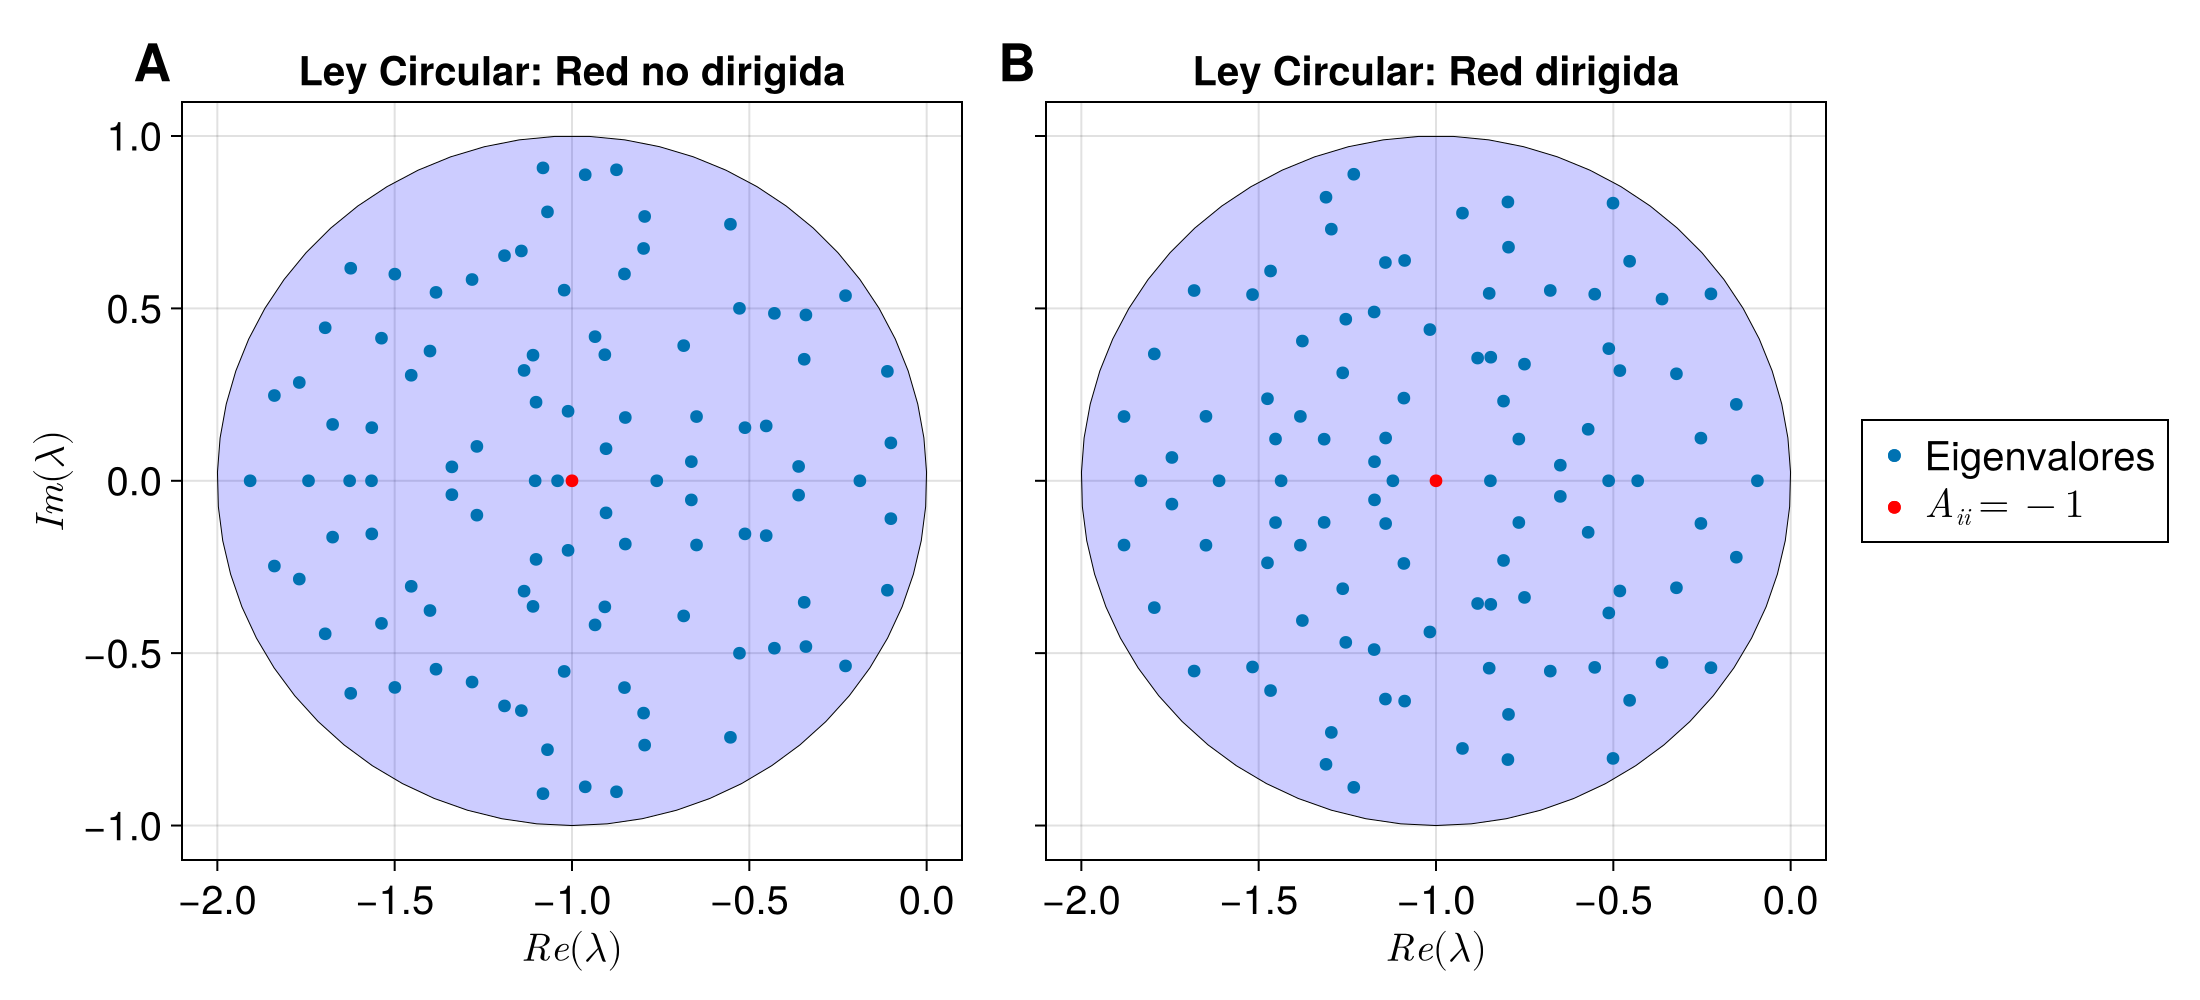
\includegraphics[scale=0.13]{../Texto/Imagenes/LeyCircularMay}
  	\caption{Distribución de eigenvalores que cumplen la Ley Circular de May. Para ambos sistemas se consideró $N=100$, una FDP normal centrada en $\mu=0$ y con $\sigma=0.2$ para una conectancia $C=\frac{1}{\sigma^2 N}-0.03$. (\textbf{A}) Considerando una matriz de interacciones estructuralmente simétrica. (\textbf{B}) Considerando una matriz de interacciones puramente aleatoria.}
  	\label{fig:LeyCircularMay}
  \end{figure}
\end{frame}
\begin{frame}
  \frametitle{Resultado de Allesina}
  Ley Elíptica
  \begin{figure}[h!]
  	\centering
  	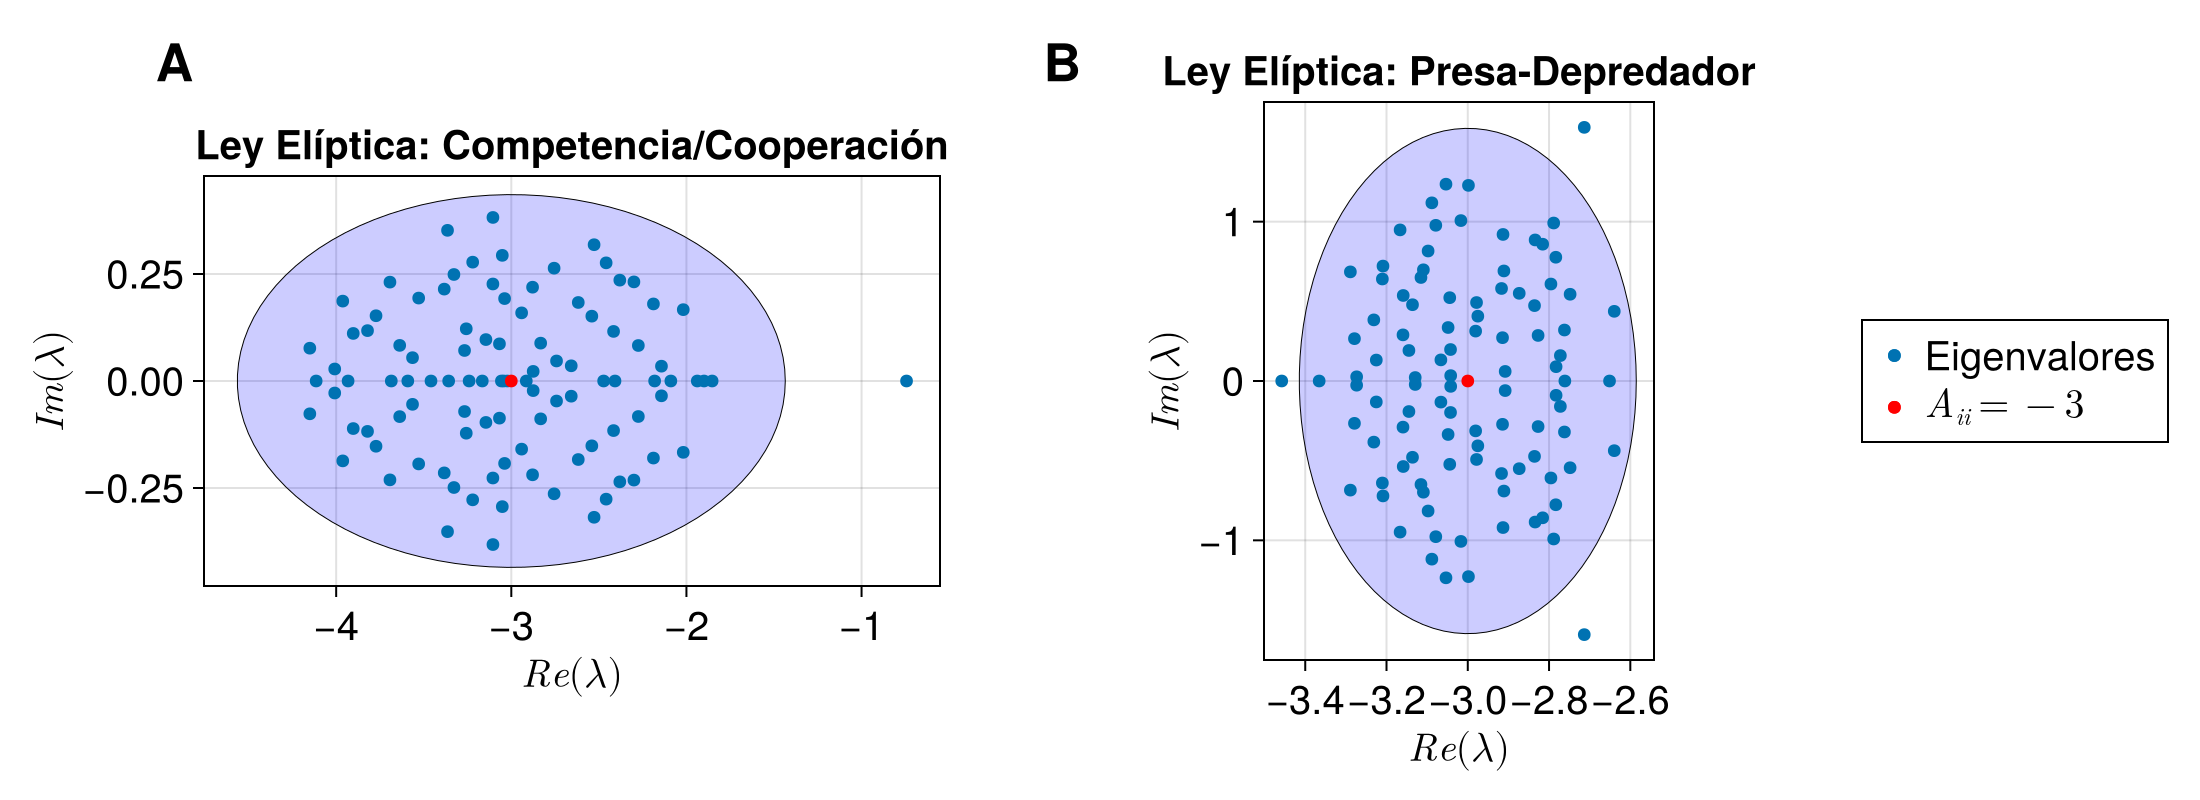
\includegraphics[scale=0.10]{../Texto/Imagenes/LeyElipticaAllesina}
  	\caption{Distribución de eigenvalores que cumplen la Ley Elíptica de Allesina. Para ambos sistemas se consideró $N=100$, dos FDP normal respectivamente, una conectancia $C=0.12$ y en ambas se debe de considerar a la matriz de interacciones como estructuralmente simétrica. (\textbf{A}) Se considera una FDP normal para la parte triangular superior con $\mu_1=0.1$ y $\sigma_1 = 0.1$ y para la parte inferior se considera otra FDP normal con $\mu_2=0.3$ y $\sigma_2 = 0.2$. (\textbf{B}) Se considera una FDP normal para la parte triangular superior con $\mu_1=-0.1$ y $\sigma_1=0.1$ y para la parte inferior se considera otra FDP normal con $\mu_2=0.3$ y $\sigma_2=0.2$. }
  	\label{fig:LeyElipticaAllesina}
  \end{figure}
\end{frame}
\begin{frame}
  \frametitle{Transiciones de May}
  Define un parámetro de transición como: $\sigma<(nC)^{-1/2}$
  \begin{figure}[h!]
  	\centering
  	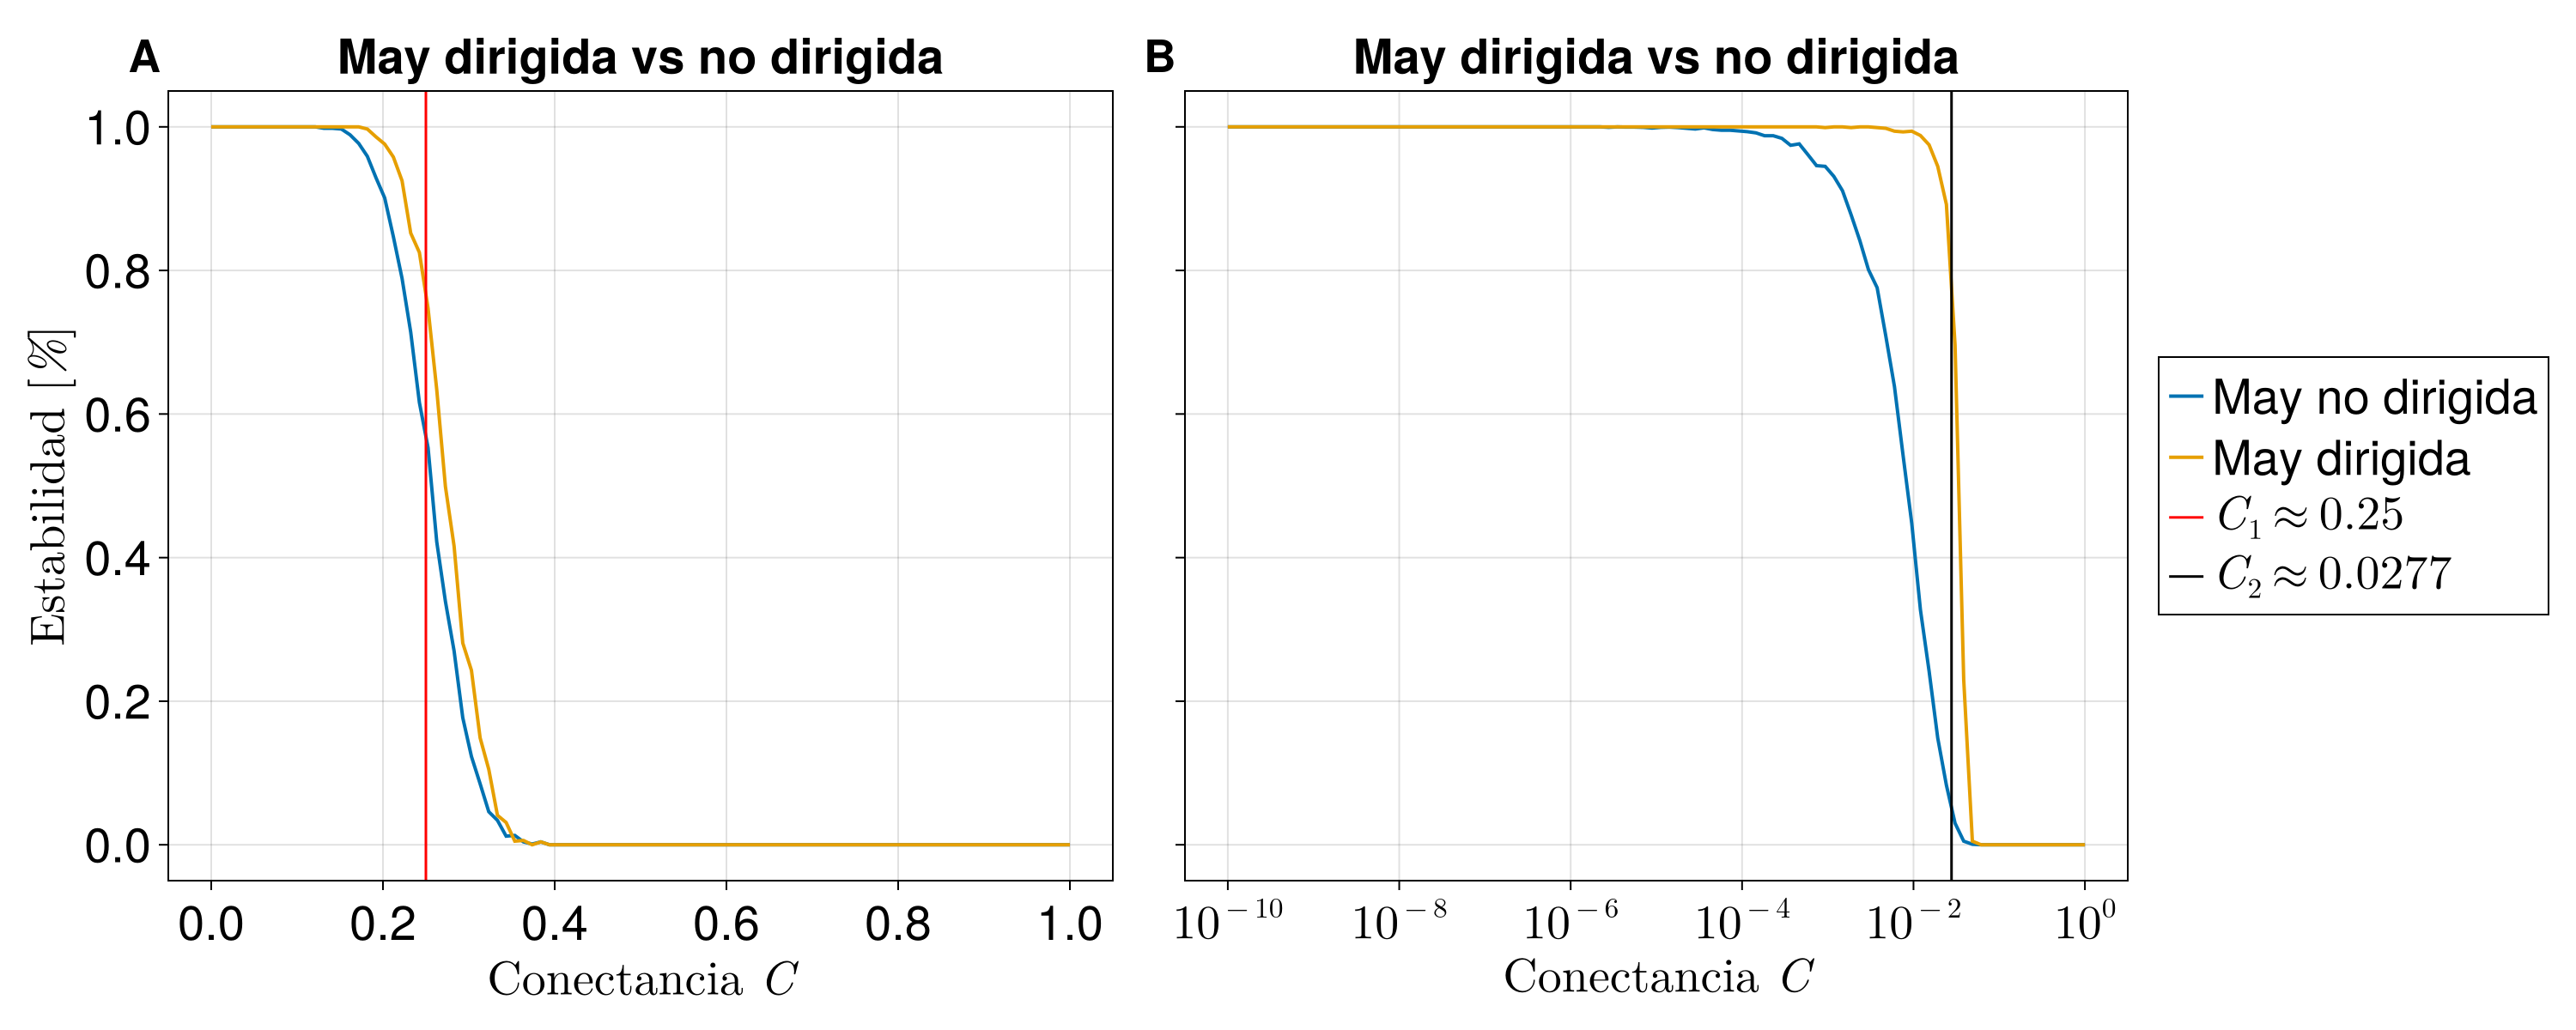
\includegraphics[scale = 0.10]{../Texto/Imagenes/TransicionDirvsNoDir}
  	\caption{Transición entre redes de May dirigidas vs No dirigidas. (\textbf{A}) Se considera para $\sigma = 0.2$ (\textbf{B}) Se considera para $\sigma=0.6$.}
  	\label{fig:TransicionDirvsNoDir}
  \end{figure}
\end{frame}
\begin{frame}
  \frametitle{Transiciones de May}
  Transición en función de $\sigma$
  \begin{figure}[h!]
  	\centering
	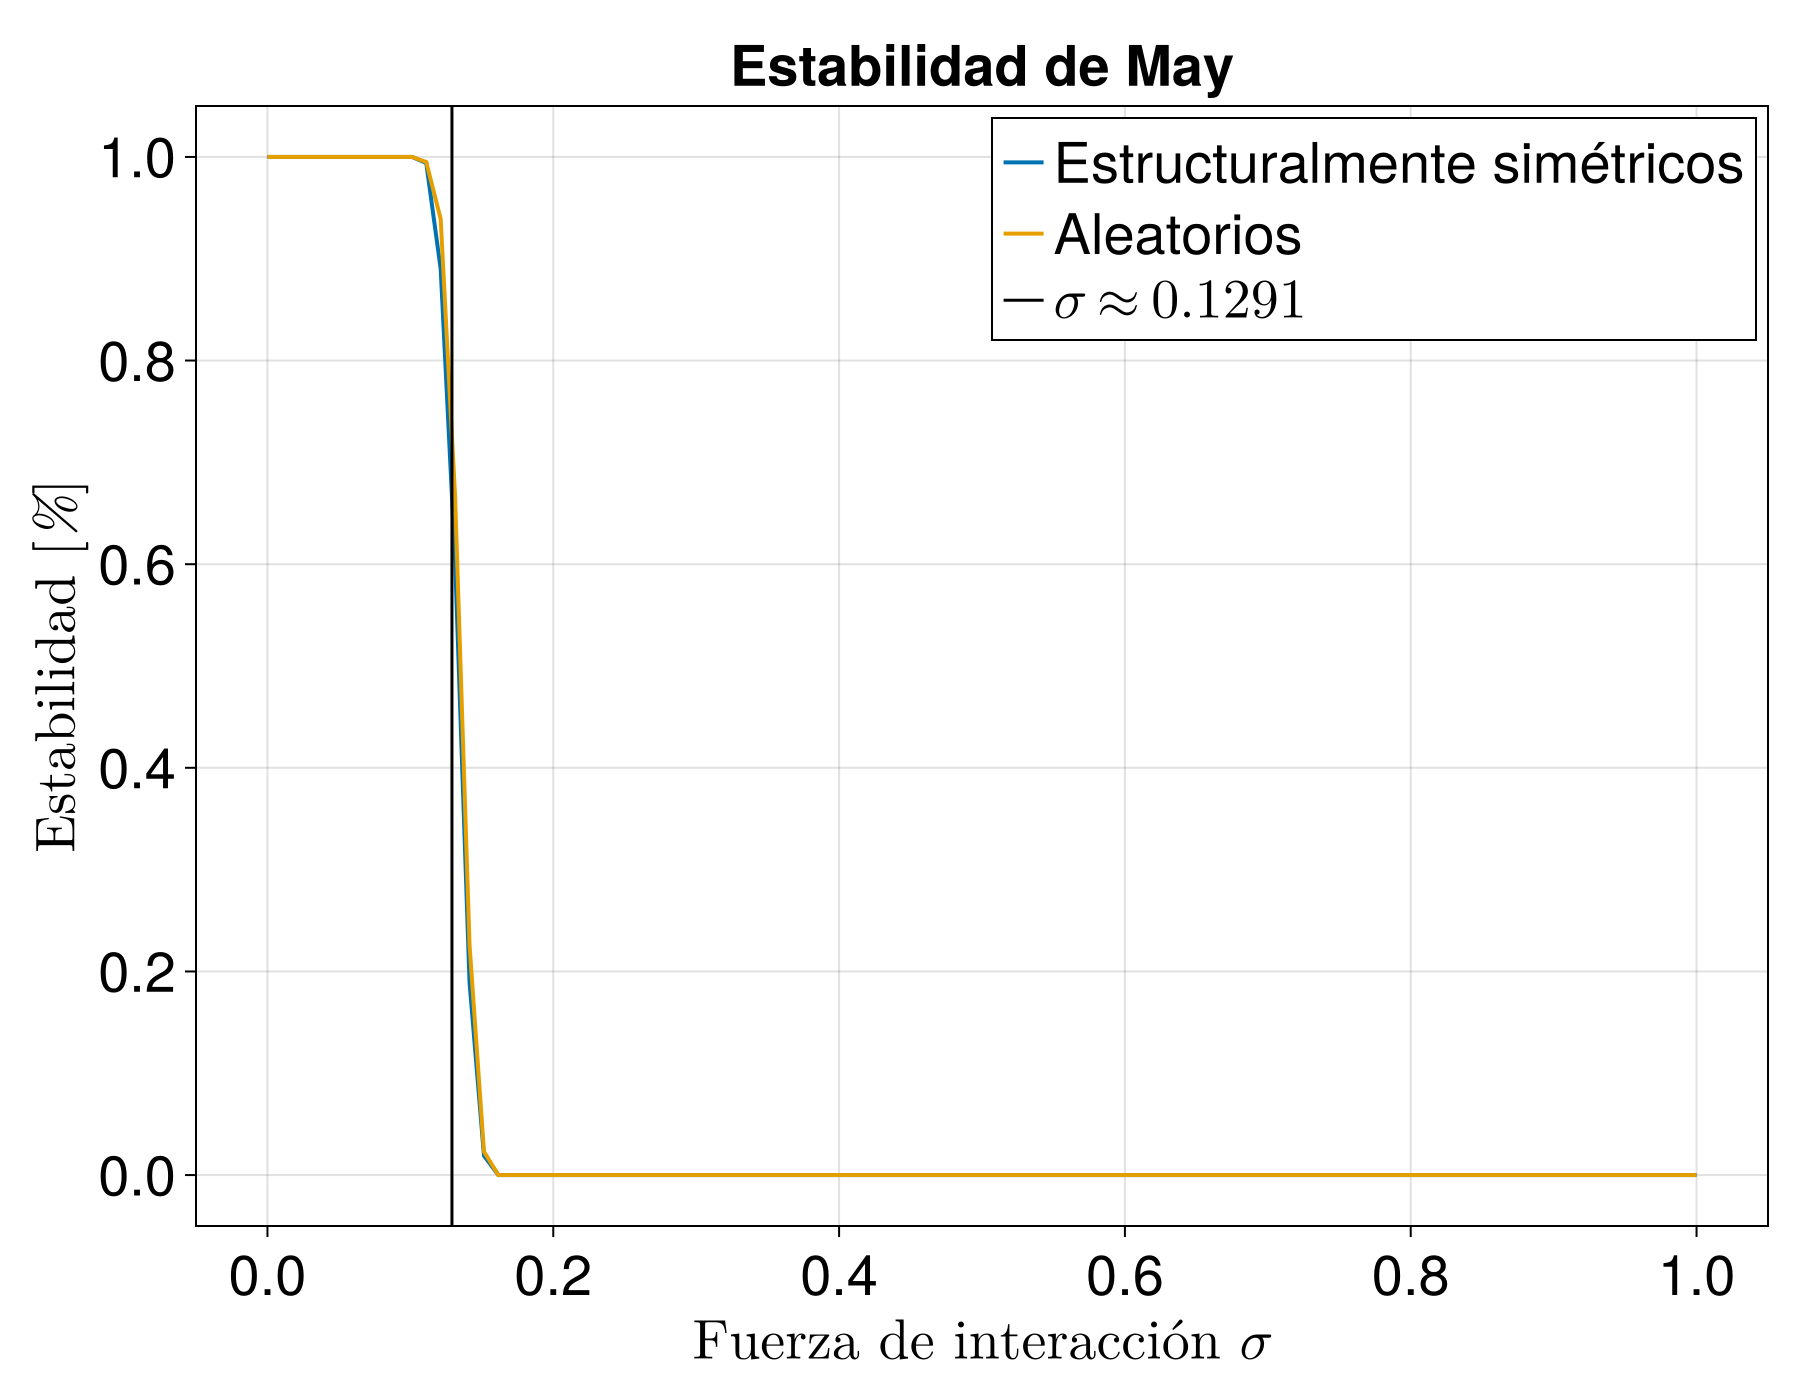
\includegraphics[width=0.52\textwidth]{../Texto/Imagenes/TransicionσDirvsNoDir} 
  	\caption{Variaciones en la transición para la matriz de May estructuralmente simétrica y para matriz puramente aleatoria. Se consideró el valor de la conectancia $C=0.6$.} 
  	\label{fig:TransicionσDirvsNoDir}
  \end{figure} 
\end{frame}
\begin{frame}
  \frametitle{Test}
\end{frame}
\begin{frame}
  \frametitle{Test}
\end{frame}
\begin{frame}
  \frametitle{Test}
\end{frame}
\begin{frame}
  \frametitle{Test}
\end{frame}
\begin{frame}
  \frametitle{Test}
\end{frame}
\begin{frame}
  \frametitle{Test}
\end{frame}
\begin{frame}
  \frametitle{Test}
\end{frame}
\begin{frame}
  \frametitle{Test}
\end{frame}
\begin{frame}
  \frametitle{Test}
\end{frame}
\begin{frame}
  \frametitle{Test}
\end{frame}
\begin{frame}
  \frametitle{Test}
\end{frame}
\begin{frame}
  \frametitle{Test}
\end{frame}
\begin{frame}
  \frametitle{Test}
\end{frame}
\begin{frame}
  \frametitle{Test}
\end{frame}
\begin{frame}
  \frametitle{Test}
\end{frame}
\begin{frame}
  \frametitle{Test}
\end{frame}
\begin{frame}
  \frametitle{Test}
\end{frame}
\begin{frame}
  \frametitle{Test}
\end{frame}
\begin{frame}
  \frametitle{Test}
\end{frame}
\begin{frame}
  \frametitle{Test}
\end{frame}
\begin{frame}
  \frametitle{Test}
\end{frame}
\begin{frame}
  \frametitle{Test}
\end{frame}
\begin{frame}
  \frametitle{Test}
\end{frame}
\begin{frame}
  \frametitle{Test}
\end{frame}
\begin{frame}
  \frametitle{Test}
\end{frame}
\begin{frame}
  \frametitle{Test}
\end{frame}
\begin{frame}
  \frametitle{Test}
\end{frame}
\begin{frame}
  \frametitle{Test}
\end{frame}
\begin{frame}
  \frametitle{Test}
\end{frame}
\begin{frame}
  \frametitle{Test}
\end{frame}

\end{document}
